\usetikzlibrary{mindmap}

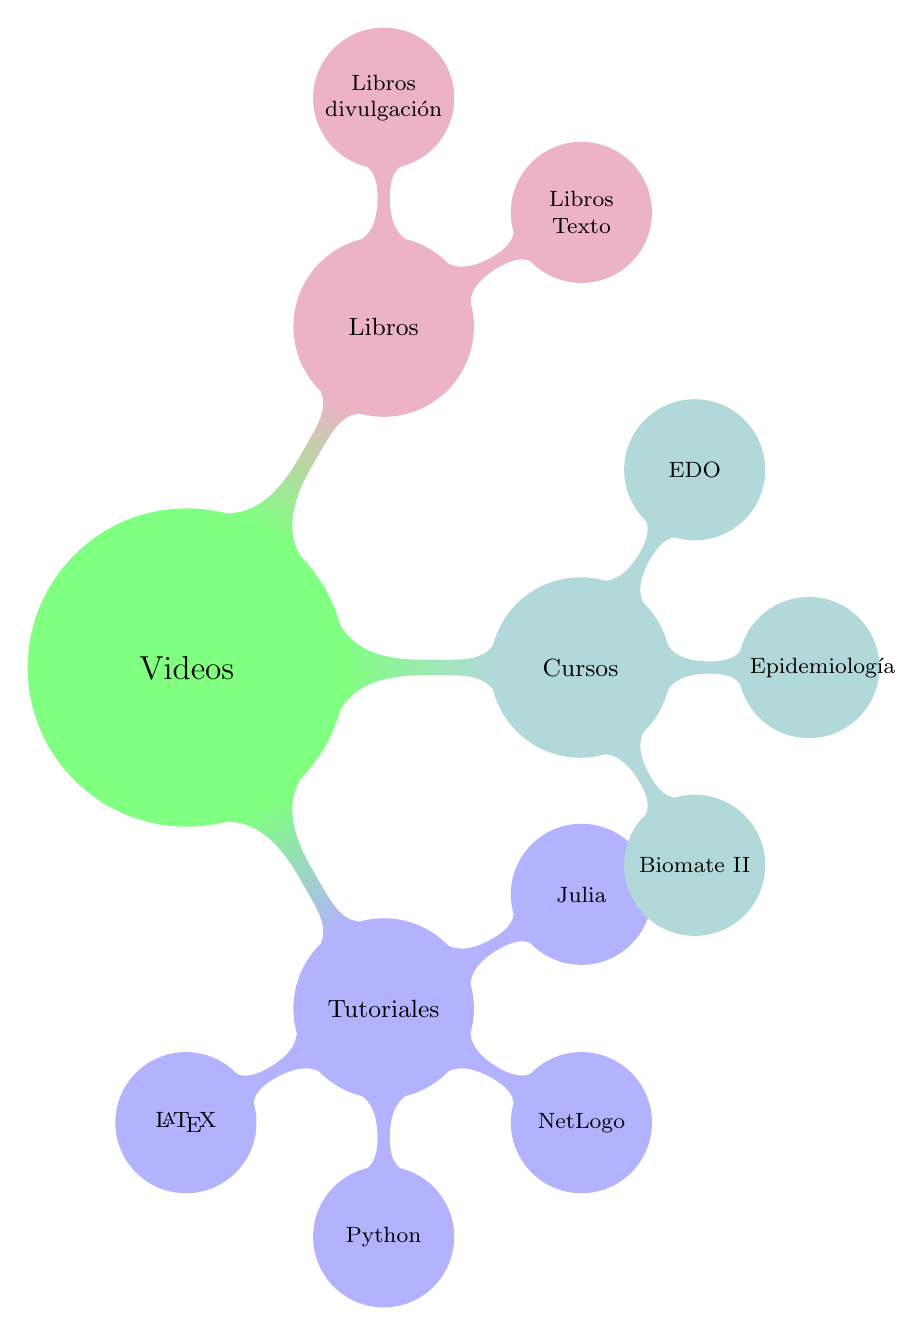
\begin{tikzpicture}[mindmap,grow cyclic,every node/.style=concept,concept color=green!50,
	level 1/.append={level distance=5cm,sibling angle=60},
	level 2/.append={level distance=3cm,sibling angle=15},]

\node{Videos}
    child[concept color=blue!30]{ node{Tutoriales}
           child {node {\LaTeX}}
           child {node {Python}}
           child {node {NetLogo}}
           child {node {Julia}}
    }
    child[concept color=teal!30]{node {Cursos}
          child{node{Biomate II}}
          child{node{Epidemiología}}
          child{node{EDO}}
    }
   child[concept color=purple!30]{node {Libros}
          child{node{Libros Texto}}
          child{node{Libros divulgación}}
    }; 
\end{tikzpicture}
